\documentclass[a4paper, 12pt]{article}
\usepackage{graphicx} % Required for inserting images
\usepackage{listings}
\usepackage{parskip}

\graphicspath{{images/}}
\DeclareGraphicsExtensions{.pdf,.png,.jpg}

\lstset{tabsize=2,
    breaklines,
    columns=fullflexible,
    flexiblecolumns,
    numbers=left,
    numberstyle={\footnotesize},
    extendedchars=\true
}
\lstdefinelanguage{command-bash}{
  sensitive=true,
  basicstyle=\small,
  morecomment=[l]{\#},
  ndkeywordstyle=\color{darkgray}\bfseries,
  identifierstyle=\color{black},
  commentstyle=\color{blue}\ttfamily,
  stringstyle=\color{red}\ttfamily,
  showstringspaces=false,
  keepspaces=true,
  escapechar=\%,
  texcl=true
}

\title{3D Viewer v2.0}
\author{sharikac, keenanbu}
\date{January 2024}


\begin{document}
\maketitle
\newpage
\begin{abstract}
\large This is a C++ program with a Qt-based interface which can visualise 3D wireframe models.
\center{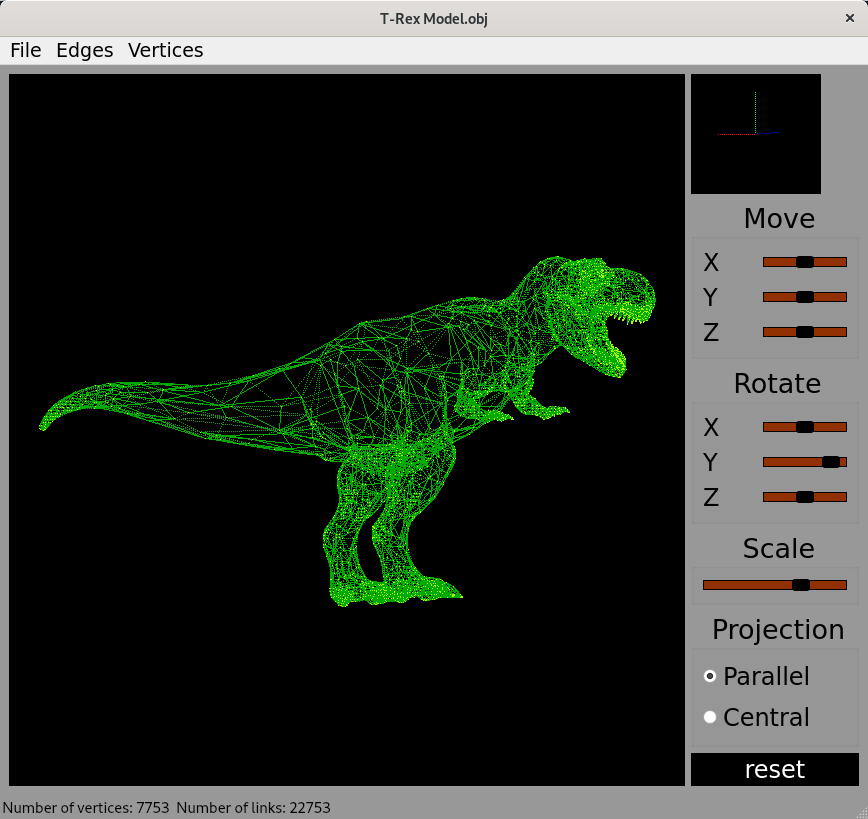
\includegraphics[width=1\textwidth]{images/3D_viewer.png}}
\newpage
{\bf \large It allows you to:}
\begin{itemize}
\item \parskip 3mm Load a wireframe model from an .obj file (vertices and surfaces list support only).
\item Translate the model by a given distance in relation to the X, Y, Z axes.
\item Rotate the model by a given angle relative to its X, Y, Z axes.
\item Scale the model by a given value.
\end{itemize}

{\bf \large \parskip 10mm The program also allows you to:}
\begin{itemize}
\item \parskip 3mm Customizing the type of projection (parallel and central)
\item Set up the type (solid, dashed), color and thickness of the edges
\item Set up the display method (none, circle, square), color and size of the vertices
\item Choose the background color
\item Save the settings between program restarts
\end{itemize}

{\bf \large \parskip 10mm It is also possible to:}
\begin{itemize}
\item \parskip 3mm Save the captured (rendered) images as bmp and jpeg files.
\item Record small screencasts by a special button - the current custom affine transformation of the loaded object into gif-animation (640x480, 10fps, 5s)
\end{itemize}
\end{abstract}

\newpage
\tableofcontents
\newpage

\section{Installation}

To install and run this program use the \textit{install} target of the Makefile:
\begin{verbatim}
make install
\end{verbatim}

To uninstall use the \textit{uninstall} target:
\begin{verbatim}
make uninstall
\end{verbatim}

\section{Making an archive}

It is possible to archive the program using the \textit{dist} target of the Makefile:
\begin{verbatim}
make dist
\end{verbatim}

\section{Running tests}

To run style tests use the \textit{style\_check} target:
\begin{verbatim}
make style_check
\end{verbatim}

To run functional tests use the \textit{test} target:
\begin{verbatim}
make test
\end{verbatim}

To check the test coverage use the \textit{gcov\_report} target. It generates an html file containing all the relevant data.
\begin{verbatim}
make gcov_report
\end{verbatim}

To check for the memory leaks use the \textit{leaks} target:
\begin{verbatim}
make leaks
\end{verbatim}

\section{Cleaning}

To clean the directory from all generated files use the \textit{clean} target of the Makefile:
\begin{verbatim}
make clean
\end{verbatim}

\newpage
\section{Using the program}

\large To load an .obj file, click on the File $\rightarrow$ Open and choose a file.
\begin{center}
  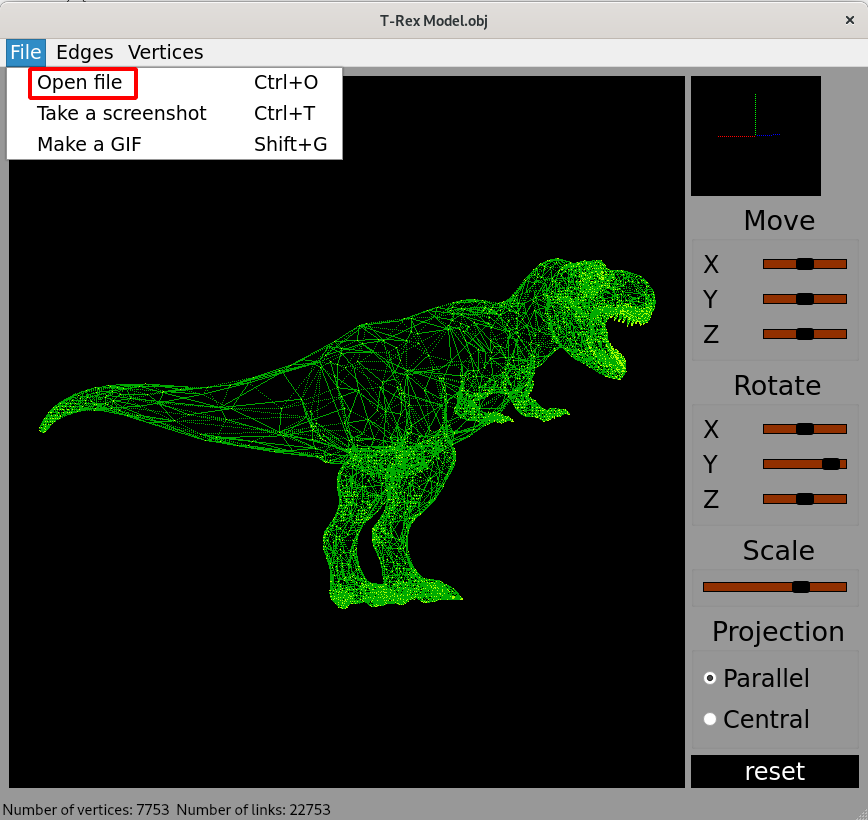
\includegraphics[width=1\textwidth]{images/open_file.png}
\end{center}

\newpage
To change the visualization settings, use the "Edges", "Vertices" and "Background" parts of the menu.
\begin{center}
  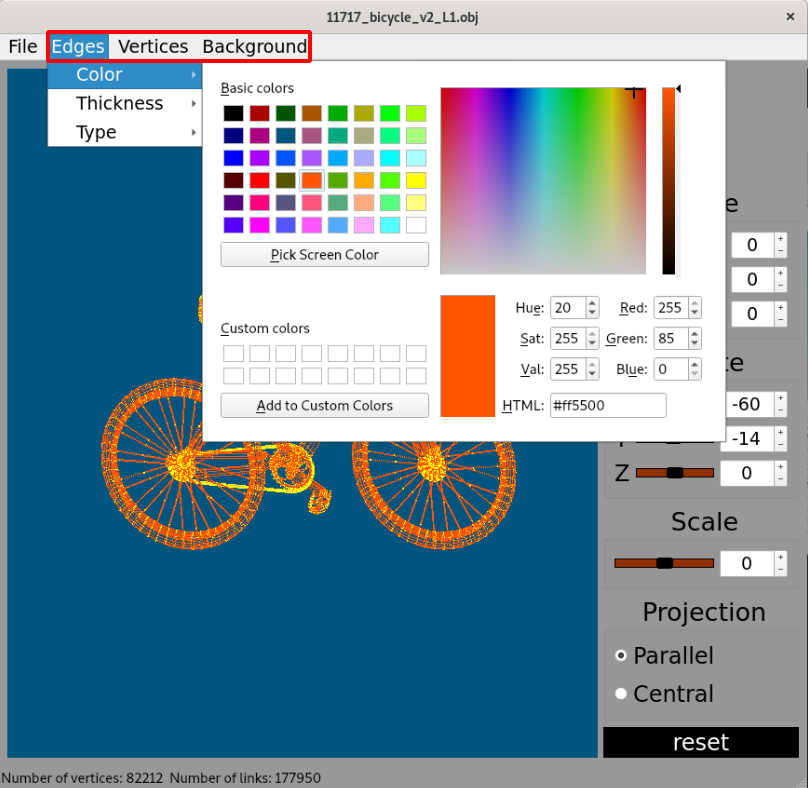
\includegraphics[width=1\textwidth]{images/color_settings.png}
\end{center}

\newpage
You can take screenshots (File $\rightarrow$ Take a screenshot) and even make 5 second GIFs recording anything happening in the rendered scene (File $\rightarrow$ Make a gif).
\begin{center}
  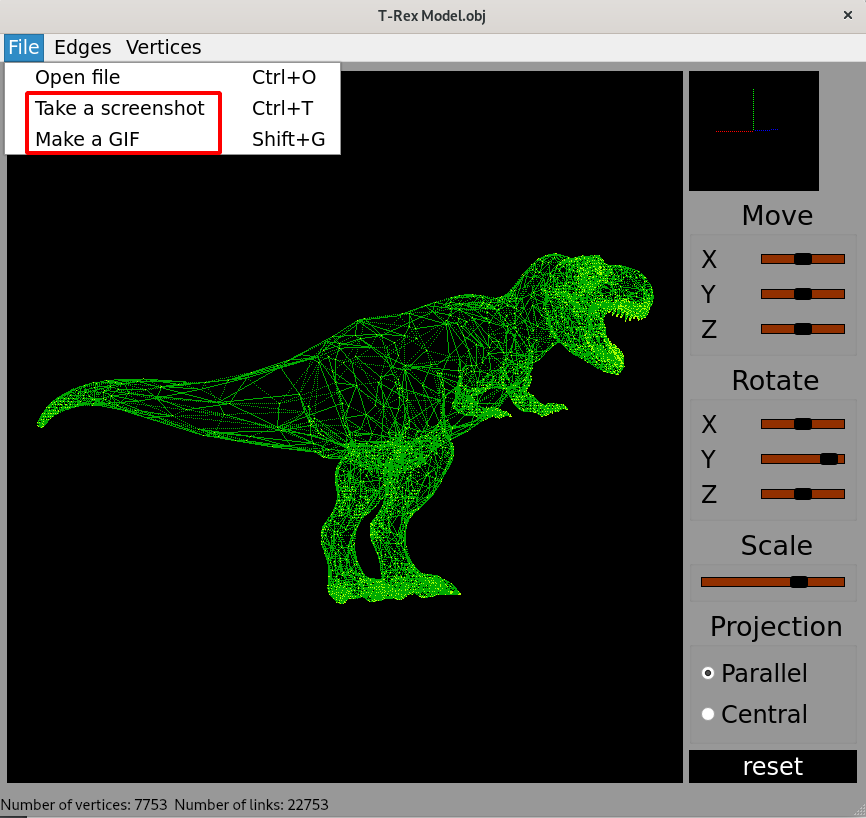
\includegraphics[width=1\textwidth]{images/screenshots_and_gifs.png}
  
\end{center}

\end{document}
